    
\chapter{Kana I}

\begin{center}
\begin{Large}
第3課: Kana I: Hiragana ひらがな  
\end{Large}
\end{center}
 
\par{ Japanese is written with a mixed script composed of four parts. Of these are two systems called \emph{Kana }. These systems spell words moraically. These means that, unlike an alphabet, every symbol will stand for a mora. Thus, a symbol may stand either for a "consonant + vowel" (CV), a "vowel" (V), or a "consonant" (C). }

\par{ The two \emph{Kana }systems are called \emph{Hiragana }and \emph{Katakana }. Because there are many symbols and rules to learn per system, we will first study \emph{Hiragana }. Then, in Lesson 3 we'll learn the symbols of \emph{Katakana }. After we've covered both sets, we'll learn about \emph{Kanji }, which are Chinese characters used in Japanese writing. }

\par{\textbf{Curriculum Note }: Just as has been the case for the past two lessons, pitch notes will be provided for the vocabulary used. High pitch is designated as text in bold. Pitch falls are noted with a ↓. }
      
\section{Hiragana ひらがな}
 
\par{\emph{K ana }represent the morae of Japanese. As we learned in Lesson 1, a mora is an equal time unit of speech . \emph{Kana }can be organized into a chart called the \emph{G }\emph{ojūo }\emph{nzu }, which means the table of 50 sounds. Although it doesn't actually have 50 sounds in it, they are deemed to be the most basic sound combin ations in Japanese, which are called \emph{seion }. }

\par{ Each \emph{Kana }system has its own set of symbols. That means once you have mastered the \emph{Hiragana }symbols below, you'll have to prepare yourself to learn an entirely different set for the same sound combinations. As tedious as this might seem, the two systems are used differently. The most important and most used system is \emph{Hiragana }, which is why it is being introduced to you first. }

\par{\textbf{\emph{HIRAGANA }}}

\par{ The basic symbo ls of \emph{Hiragana }, as stated above, are organized into a chart called the \emph{Gojūonzu }. This chart is shown below with each basic symbol. Notice how the chart is organized. Stoke orders are listed, and all the allophones of sounds we learned in the previous lesson are shown in their respective columns. }
 
\begin{figure}[h]
\centering

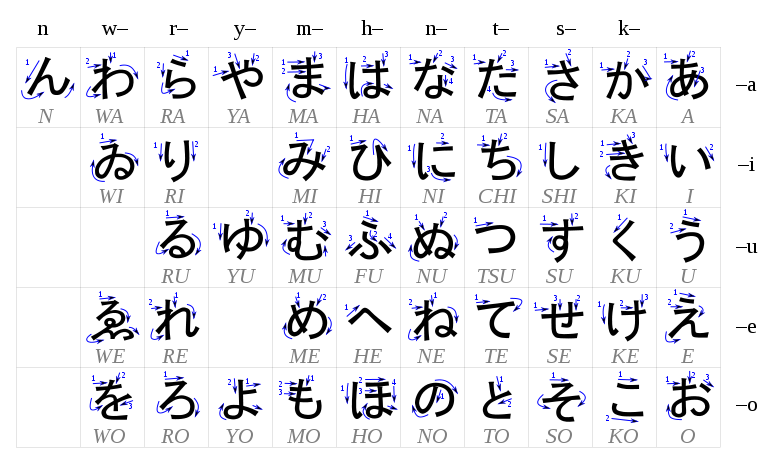
\includegraphics[width=0.9\textwidth]{figs/第01章/第3課:_hiragana_fig/768px_Table_hiragana.svg.png}

\end{figure}

\par{\textbf{Curriculum Note }: Print this sheet out and have it at hand as we continue moving forward. After we've learned about \emph{Katakana }and Chinese characters ( \emph{Kanji }), we'll learn how they're all three used along with English letters to write Japanese. }

\par{\textbf{Usage Notes }: }

\par{Of these characters, all except the symbols for \emph{we }and \emph{wi }\emph{ }are actually used. These two characters live on only in names, place names, and old literature. Because there is the chance you will encounter them, when you do see them, read them as "e" and "i" respectively as the "w" has dropped from their actual pronunciations. This is largely why the symbols are no longer seen today. }

\par{ Similarly, the symbol for \emph{wo }is usually pronounced by "o" by most speakers. However, the traditional pronunciation "wo" is still heard depending on personal preference, dialect, as well as occasion. For instance, in music, singers tend to be conservative in pronunciation. This is also the case when people slow down their speech to purposefully enunciate every sound clearly. }

\par{ Of these characters, all but the symbols for \emph{we }, \emph{wi }, \emph{wo }, and \emph{n }can start words. Also, the symbol for \emph{wo }is only used in names or as a grammatical word that cannot stand alone, which we will learn about later. }

\par{\textbf{Handwriting Notes }: }

\par{1. Write strokes from top to bottom and left to right. \hfill\break
2. Make sure the end of the second stroke in あ is crossing the curve of the final stroke. \hfill\break
3. Make sure that the final stroke in け is slightly farther down than the first. \hfill\break
4. For せ, the second stroke usually doesn't have a hook. \hfill\break
5. For い, こ, た, ふ, り, and ゆ, don't connect the strokes together. \hfill\break
6. For む, if you connect stroke 2 and 3, do not add another slash. \hfill\break
7. Make sure the stroke 3 for お is not positioned far away from the rest of the character. \hfill\break
8.  In more proper handwriting, the last stroke in さ and き is not connected  with the rest. }

\begin{center}
Examples 
\end{center}

\par{ The best way to see if you can read \emph{Hiragana }is to practice with actual words. Below is a list of 30 common words written without any aids. }

\begin{ltabulary}{|P|P|P|P|P|P|}
\hline 

Shape & か \textbf{たち }& Dream & ゆ \textbf{め }↓ & Japan & に \textbf{ほ }ん \\ \cline{1-6}

Usual & ふ \textbf{つう }& End & お \textbf{わり }& Promise & や \textbf{くそく }\\ \cline{1-6}

Snow & ゆ \textbf{き }↓ & Kitten & こ \textbf{ね }こ & Proof & あ \textbf{かし }\\ \cline{1-6}

Chair & い \textbf{す }& Bowl & う \textbf{つわ }& Plate & さ \textbf{ら }\\ \cline{1-6}

Payment & し \textbf{はらい }& Seat &  \textbf{せ }き & Speculation & す \textbf{いそく }\\ \cline{1-6}

Gymnasium & た \textbf{いいく }かん & Strength & ち \textbf{から }↓ & Pathway &  \textbf{つ }うろ \\ \cline{1-6}

Store clerk & て \textbf{んいん }& Chicken meat & と \textbf{りにく }& Accent & な \textbf{まり }↓ \\ \cline{1-6}

Duty &  \textbf{に }んむ & Bypath & ぬ \textbf{けみち }& Drink & の \textbf{み }もの \\ \cline{1-6}

Secret & ひ \textbf{みつ }& Star & ほ \textbf{し }& Command & め \textbf{いれい }\\ \cline{1-6}

Night &  \textbf{よ }る & Young person & わ \textbf{かもの }& Bus\slash train line & ろ \textbf{せん } \\ \cline{1-6}

\end{ltabulary}

\begin{center}
\textbf{Diacritics: ゛ \& ゜ }
\end{center}

\par{ There are two diacritics that can be added to symbols that change the consonant of the symbol in question. These diacritics are the ゛ ( \emph{da \textbf{kuten }\slash ni \textbf{gori }}↓) and the ゜ ( \emph{ha \textbf{ndakuten }}). The first diacritic changes a consonant into a voiced consonant. A voiced consonant causes the vocal folds to vibrate. The second diacritic changes \slash h\slash  to a \slash p\slash . }
 
\begin{figure}[h]
\centering

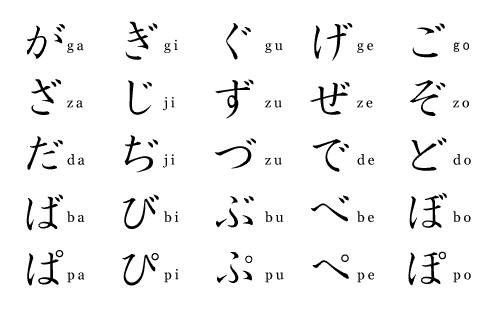
\includegraphics[width=0.9\textwidth]{figs/第01章/第3課:_hiragana_fig/Hiragana_dakuten_chart.png}

\end{figure}
\hfill\break

\par{ When writing these characters, you write the diacritics last. It's important to note how there are two characters for \slash ji\slash  and \slash zu\slash . These symbols are not always pronounced exactly the same, but we will go into greater detail about this later. }

\begin{center}
Examples 
\end{center}

\par{ The hardest part to mastering the diacritics will simply be remembering to use them and realizing that the pronunciation of a symbol will change because of them. For practice, below are 30 common words that utilize them. }

\begin{ltabulary}{|P|P|P|P|P|P|}
\hline 

Number &  \textbf{か }ず & College student & だ \textbf{いが }くせい & Key & か \textbf{ぎ }↓ \\ \cline{1-6}

Walk & さ \textbf{んぽ }& Mountain climbing &  \textbf{と }ざん & Culture &  \textbf{ぶ }んか \\ \cline{1-6}

Throat &  \textbf{の }ど & Poison & ど \textbf{く }↓ & Yes and no &  \textbf{さ }んぴ \\ \cline{1-6}

Cheers & か \textbf{んぱい }& Nosebleed & は \textbf{なぢ }& Attachment &  \textbf{て }んぷ \\ \cline{1-6}

Electricity &  \textbf{で }んき & Potentiality & そ \textbf{こぢ }から & Hippopotamus &  \textbf{か }ば \\ \cline{1-6}

Skin &  \textbf{は }だ & Furniture &  \textbf{か }ぐ & Wall & か \textbf{べ }\\ \cline{1-6}

Elbow & ひ \textbf{じ }↓ & Part &  \textbf{ぶ }ぶん & Whirlpool &  \textbf{う }ず \\ \cline{1-6}

Continuation & つ \textbf{づき }& Scale &  \textbf{き }ぼ & Wind & か \textbf{ぜ }\\ \cline{1-6}

Eyelash & まつげ & Crevice & ひ \textbf{びわれ }& Tatami room & ざ \textbf{しき }↓ \\ \cline{1-6}

Mirror & か \textbf{がみ }↓ & Family &  \textbf{か }ぞく & Map &  \textbf{ち }ず \\ \cline{1-6}

\end{ltabulary}

\begin{center}
\textbf{Palatal Sounds }
\end{center}

\par{ Palatal sounds are created by placing the tongue on the hard palate of the mouth. Many consonants in Japanese can be palatalized and then followed by the vowels \slash a\slash , \slash i\slash , \slash u\slash , and \slash o\slash . In the case of \slash i\slash , palatalization is an inherent part of the pronunciation of the sound combination. For instance, \slash ki\slash , \slash shi\slash , \slash chi\slash , \slash ni\slash , \slash mi\slash , \slash hi\slash , and \slash ri\slash  are all technically palatalized. This is simply part of the natural process of pronouncing them. }

\par{ The way Japanese creates more sound combinations with palatalized combinations is by having \slash ya\slash , \slash yu\slash  and \slash yo\slash  follow a consonant. When this happens, new consonants are produced. In \emph{Hiragana }, these combinations are created by using an i-sound symbol with a shrunken y-sound symbol-- ゃ, ゅ, or ょ. }

\begin{figure}[h]
\centering

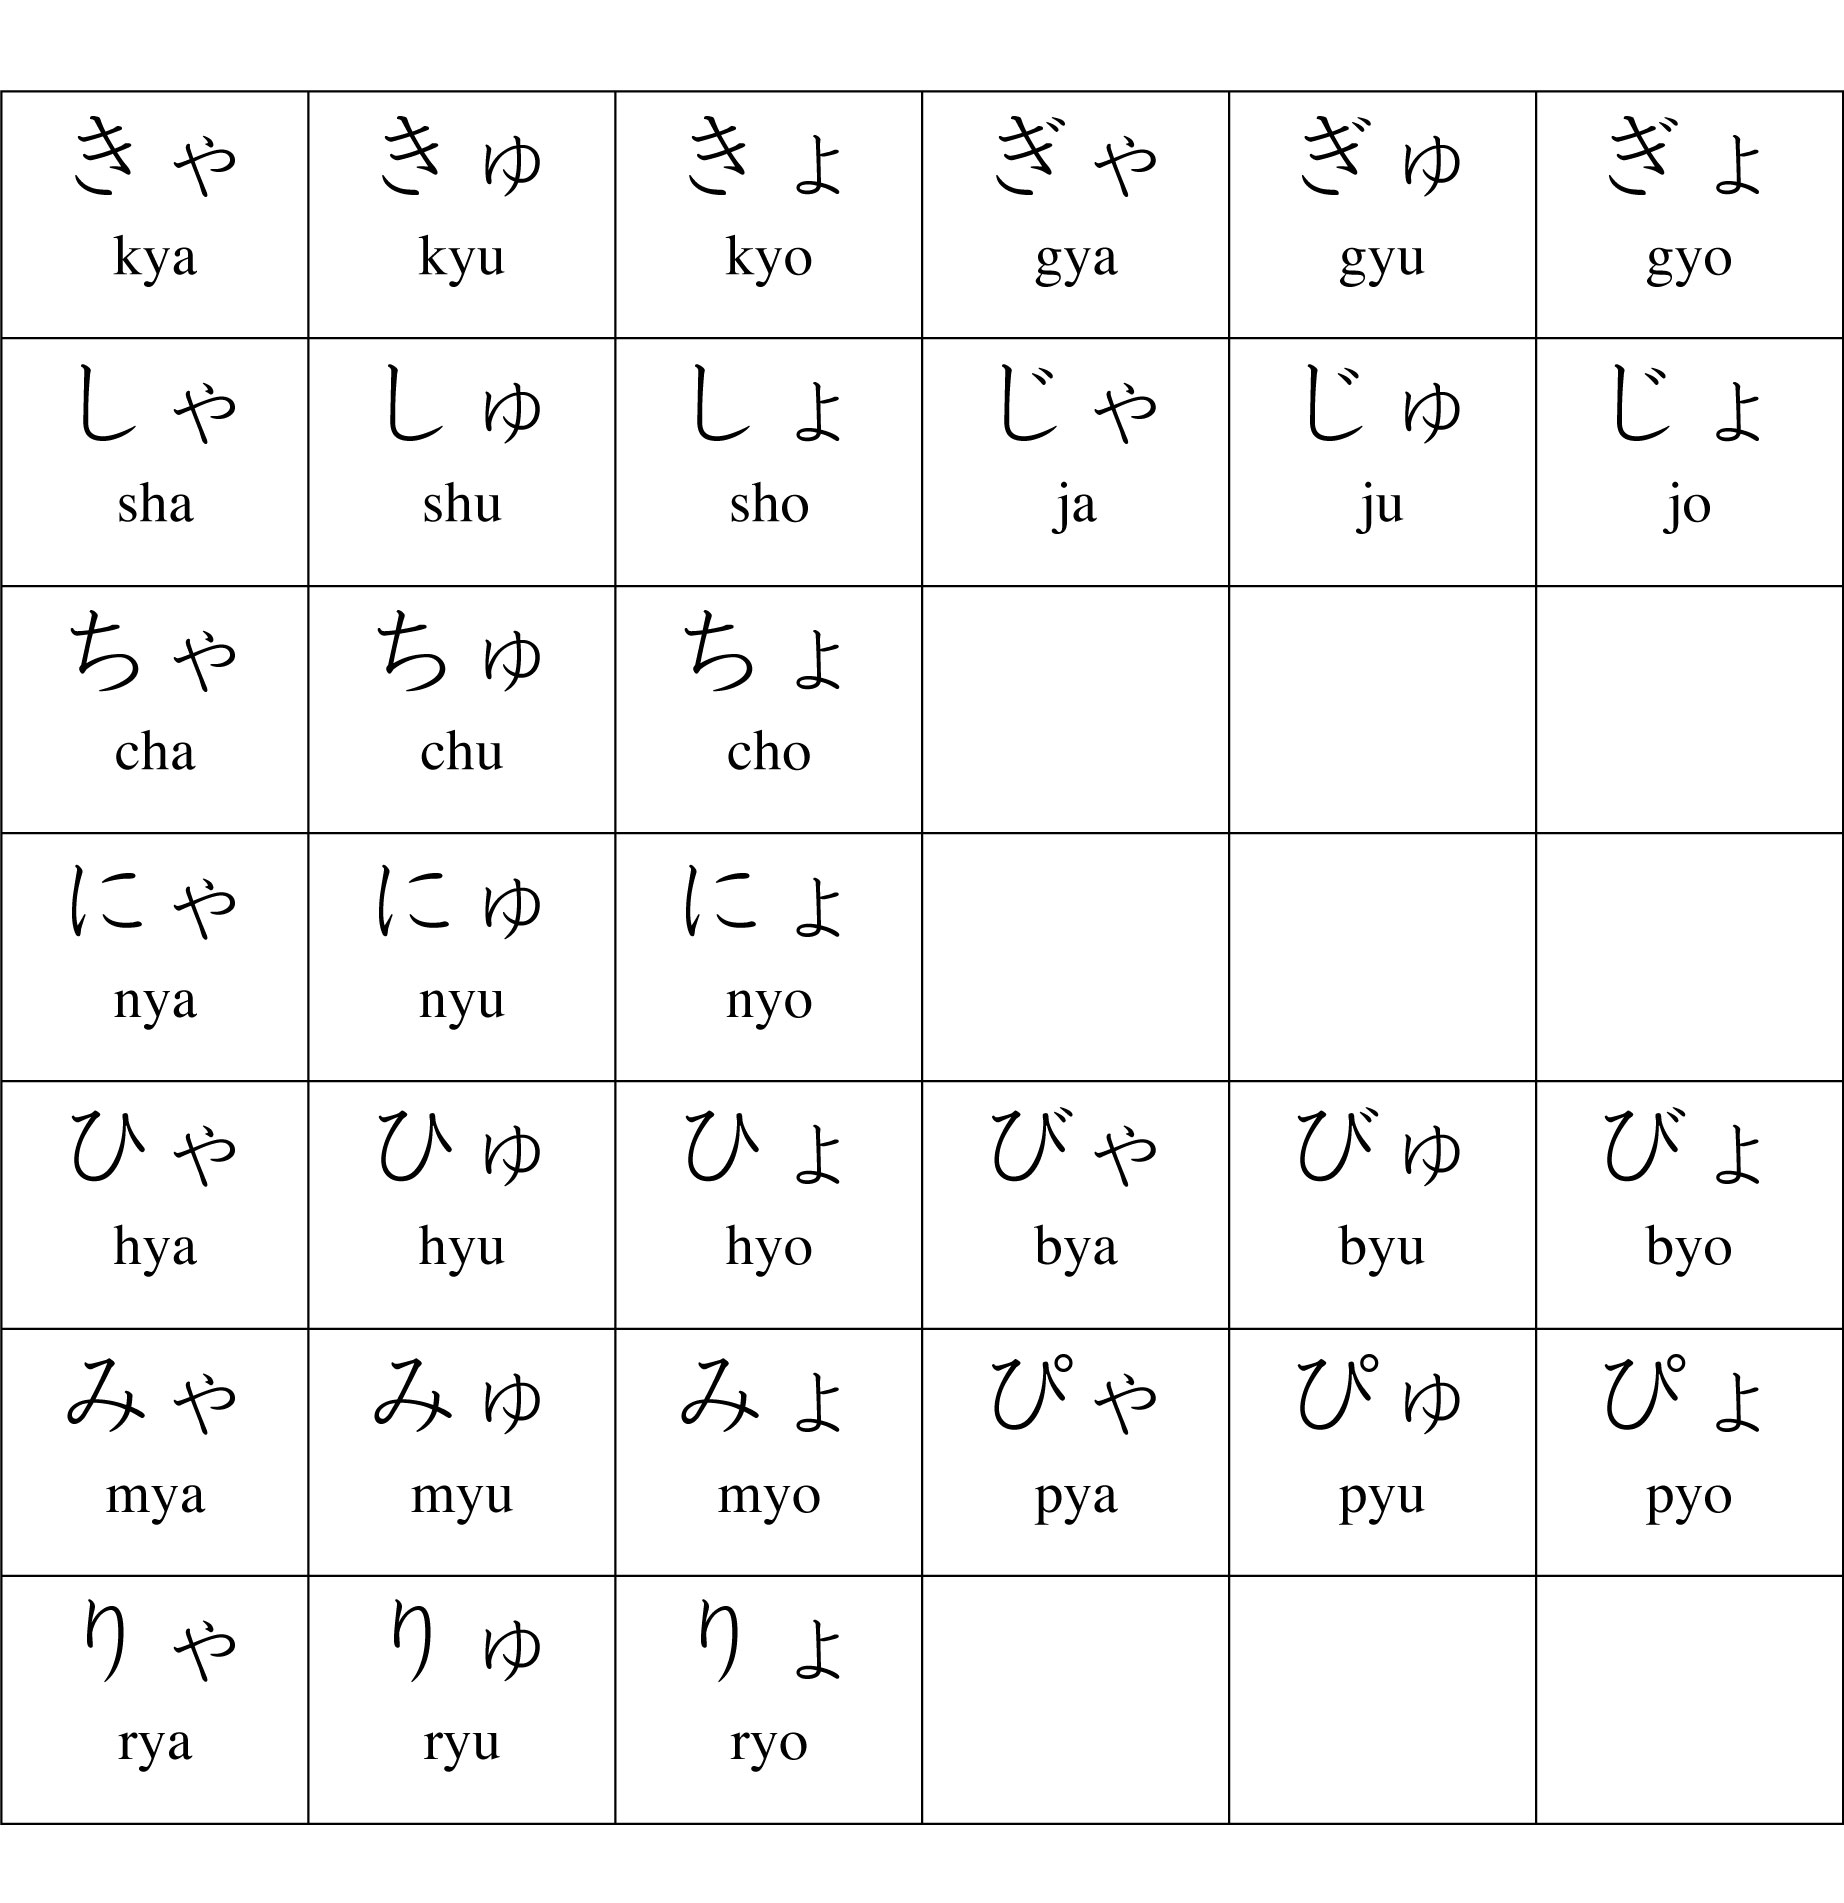
\includegraphics[width=0.9\textwidth]{figs/第01章/第3課:_hiragana_fig/hiragana03.png}

\end{figure}
 
\par{ Similarly to above, there are two ways to write \slash ja\slash , \slash ju\slash , and \slash jo\slash . For now, we'll put aside how they differ in pronunciation and usage and solely focus on memorizing these glyphs. Note, though, that you will rarely see the variants that utilize ぢ. }

\par{ Pronunciation-wise, the ry-sounds will be the most difficult to master as the Japanese \slash r\slash  tends to be difficult as it is for native English speakers to acquire. }

\begin{center}
Examples  
\end{center}

\par{ Below are 30 words utilizing these glyphs to help you learn them. }

\begin{ltabulary}{|P|P|P|P|P|P|}
\hline 

Resident & じゅ \textbf{うみん }& Parking \hfill\break
Injection & ちゅ \textbf{うしゃ }& Giant & きょ \textbf{じん }\\ \cline{1-6}

Meow-meow &  \textbf{にゃ }ん \textbf{にゃ }ん & Acronym & りゃ \textbf{くご }& Tune \hfill\break
& きょ \textbf{く }\\ \cline{1-6}

Seafood & ぎょ \textbf{か }いるい & Inn & りょ \textbf{かん }& Opposite & ぎゃ \textbf{く }\\ \cline{1-6}

600 & ろっ \textbf{ぴゃく }↓ & Tathagata & にょ \textbf{らい }& Studying abroad & りゅ \textbf{うがく }\\ \cline{1-6}

Cow milk & ぎゅ \textbf{うにゅう }& Bathing & にゅ \textbf{うよく }& Customer & きゃ \textbf{く }\\ \cline{1-6}

Concentration & しゅ \textbf{うちゅ }うりょく & Processing &  \textbf{しょ }り & Society &  \textbf{しゃ }かい \\ \cline{1-6}

Touch down & ちゃ \textbf{くりく }& Tea & お \textbf{ちゃ }& Directly & ちょ \textbf{くせつ }\\ \cline{1-6}

Weak point & じゃ \textbf{くて }ん & Tutor & じょ \textbf{しゅ }& Pulse & みゃ \textbf{く }↓ \\ \cline{1-6}

Teacup & ゆ \textbf{のみぢゃ }わん & Hyuga &  \textbf{ひゅ }うが & 100 & ひゃ \textbf{く }↓ \\ \cline{1-6}

Chinese & ちゅ \textbf{うごくご }& Properly & ちゃ \textbf{んと }& Address &  \textbf{じゅ }うしょ \\ \cline{1-6}

\end{ltabulary}
\hfill\break
 Although it may be difficult to properly pronounce these palatal sounds, mispronouncing them as separate morae will result in the word either becoming a different word altogether or a non-word. \hfill\break
\hfill\break

\begin{ltabulary}{|P|P|}
\hline 

i-sound + や・ゆ・よ & i-sound + ゃ・ゅ・ょ \\ \cline{1-2}

じ \textbf{ゆ }う (Freedom) &  \textbf{じゅ }う  (Ten\slash gun) \\ \cline{1-2}

り \textbf{ゆう }(Reason) &  \textbf{りゅ }う (Dragon) \\ \cline{1-2}

き \textbf{\emph{ゆ }う }(Needless anxiety) &  \textbf{きゅ }う (Nine) \\ \cline{1-2}

し \textbf{ゆう }(Private ownership) &  \textbf{しゅ }う (Week\slash state) \\ \cline{1-2}

\end{ltabulary}
\hfill\break

\begin{center}
 \textbf{To Continue }
\end{center}

\par{ So far, we have covered the unique glyphs that compose \emph{Hiragana }. What we have not learned is how long consonants and vowels are transcribed. We have also not learned about what situations \emph{Hiragana }is even used in. Both of these topics require that we first go over \emph{Katakana }as comparing the two is essentially in understanding these topics properly. }

\begin{center}
\textbf{Practice } 
\end{center}

\par{Part I: Change the following words into \emph{Hiragana }. }

\par{1. \emph{Ke \textbf{muri }}(smoke) \hfill\break
2. \emph{A \textbf{magumo }}(rain cloud) \hfill\break
3. \emph{U }\textbf{\emph{ta }↓ }(song)  \hfill\break
4. \emph{\textbf{Se }kai }(world) \hfill\break
5. \emph{Ka \textbf{rate }} (karate)   }

\par{Part II: Change the following words in \emph{Hiragana }into \emph{Rōmaji }. }

\par{1. \textbf{か }のじょ (She)  2. しょ \textbf{だな }(Bookshelf) \hfill\break
3. に \textbf{ほんご }(Japanese language)  4. さ \textbf{かな }(Fish) \hfill\break
5. に \textbf{んげん }(Human)  6. だ \textbf{いがく }(College) \hfill\break
7. ひ \textbf{と }(Person)  8. あ \textbf{した↓ }(Tomorrow)  }
    